\chapter{协作改进整个系统} % Introduction chapter suppressed from the table of contents

``专注用户，从顾客的角度生产产品。''\\
某次现场培训，我分享了丰田汽车故事后，请学员分组讨论，写出对工作最有帮助的3条。以上是某组的第一条，我请他们解释说明。\\
``我是做开发的，反思时发现其实不清楚我的工作对客户有什么作用。''一位年轻的编码人员说。\\
因为编码工作大部分都是由产品经理或项目经理过滤后分配，所以如果你随便问身边的编码人员，70-80\%的可能不知道用户为什么要这样做，要开发的功能有什么价值。\\
这位年轻编码人员的分享让我想到2年前某公司要推行需求与研发分离的故事。

\hypertarget{ux9700ux6c42ux4e0eux7814ux53d1}{%
\subsection{需求与研发}\label{ux9700ux6c42ux4e0eux7814ux53d1}}

质量部经理：以前需求是研发团队的一部分，很多时候就会倾向于从研发团队的角度来看需求。公司希望分开后可以更加独立，更多地从客户的视角看需求，也希望需求可以与研发相互制衡。\\
我：你们把需求与开发分家以后有没有遇到什么问题？\\
质量部经理：遇到问题可不少，例如研发团队会说------需求人员把需求写得太简单了，写得不清楚，无法开发。而需求人员却说，要写到多详细才可以开发，你可以给我一个标准吗？甚至有些较极端的研发人员，明知需求有问题，但是还是按需求的描述做开发。公司领导希望利用标准化流程和相关度量指标去控制过程。我就是负责制定这些指标的，但有个问题，比如我们觉得研发做出来的产品应该得到客户的认同、让客户满意。所以客户满意度应该很重要。但研发组长就拒绝了这指标，他说------现在我们只做研发，不负责需求，也控制不了需求的质量，为什么最终那个产品的满意度要由研发负责？而如果要求需求人员对最终的客户满意度负责，体现在KPI指标，他们会说------我们只做需求，开发做出来的产品客户不满意，为什么让需求买单？\\
听起来两边都理。\\
我：如果我们希望只通过某些指标监控过程，比如代码评审缺陷率，希望提前发现错误，尽早修正，反而会影响总体效果。团队可能因花大量精力评审，影响了交付速度，反而会导致客户的不满意。如果客户对产品不满意，开发肯定有问题，所以只追求某些过程指标没有意义。人很聪明，会想出各种满足指标的方法。\\
例如管理层希望加强代码评审改善产品质量，开会时跟开发与测试人员说：``如果评审的缺陷数量能超过指标，便会按超过的数量发奖金。''\\
会后，测试不服气，私下跟开发说：``估计你们很快可以轻松地变成百万富翁了。''\\
这经典滑稽故事有点夸张，但能点出只追求指标的问题。\\
就好比如果评审或者测试的缺陷数越高奖励越多，聪明的团队可以很轻松地变成百万富翁。\\
质量部经理：我们那些团队就很懂怎么针对指标作假。\\
公司觉得今年改革之前做新产品开发项目的立项太宽松，缺乏有效的管理和监督，这导致很多新的研发项目都是没有回报或者失败，浪费了很多资源。所以现在用新方式，所有立项的研发项目，都应该由中央委员会审批才能立项和开始做，我觉得这个倒是挺好的。\\
我：你觉得好吗？\\
你听过苹果电脑(Apple)吗？苹果公司本身就是由两人创办：一位是乔布斯、另一位是沃兹(Steve
Wozniak)，沃兹本来是惠普的工程师，在1975\textasciitilde{}1976年间研发出了苹果电脑(Apple
1)，他本来希望获得惠普高层的支持，申请内部立项，但多次都被拒绝。乔布斯看到这个产品后，觉得很有市场潜力，就跟沃兹跑市场，最终获得Byte
Shop老板Paul Terrell的首张订单，购买了200套苹果电脑(Apple 1）。当时Apple
1都由沃兹手工焊接而成。创新产品都必须具备以下重要元素：

\begin{enumerate}
\tightlist
\item
  了解市场需求的人员，乔布斯就是这个角色
\item
  研发工程师沃兹\\
\end{enumerate}

两者相互合作才把苹果产品做成。如果把需求跟研发切开，估计苹果的传奇故事永远都不会诞生。正是两人的团队合作，才会有个人电脑这个新市场。\\
创新不能用传统的工厂化流程，靠一些指标去管理。\\
惠普公司很优秀，内部肯定不缺资深专家，评判指标也应该很完善，为什么沃兹的内部申请立项，多次都被拒绝？惠普一直都是专注于做度量和测量仪器，但个人电脑是全新的概念，所以单靠现有指标是无法鼓励项目创新。发明全新的东西必须是需求配合技术开发工程师，再加上与客户的接触和确认，才会成功。\\

\hypertarget{ux7f16ux7801ux4ee5ux5916}{%
\subsection{编码以外}\label{ux7f16ux7801ux4ee5ux5916}}

这不仅仅是编码与需求的问题。测试的主要目的是希望内部先发现问题，不要等到交付给客户才暴露。\\
B公司专门做餐饮系统产品，2年前为某企业提供食堂系统。因公司一直都只为餐厅、菜馆等提供系统，测试工程师专门做了研究，发现食堂与一般的餐厅不同，因为要支撑大量员工在午餐时段点餐，通常都只提供几类套餐，简化流程，所以便向产品经理提出。但他没有接纳，还是按照客户提出的系统菜单(menu)要求开发。系统交付后，过了几个月，系统最终还要改造、简化，只保留几类套餐。\\
因为需求由产品经理负责，测试人员只能按需求制定测试计划，无法影响需求，导致走了弯路，引起本来可以避免的返工。所以应赋能与前线团队，包括开发、测试等，前期让团队一起全方位地讨论给客户的价值，减少浪费。

\hypertarget{ux5c0fux7ed3}{%
\subsection{小结}\label{ux5c0fux7ed3}}

从以上3个故事看到员工只管自己负责的任务、过程，导致：

\begin{itemize}
\tightlist
\item
  团员不清楚最终对客户的效果和价值（例如开发）
\item
  每个过程的指标都很好，不一定代表总体效果会理想
\item
  容易引起各自为政
\end{itemize}

最终做不出优秀产品，
所以戴明博士的经典14点里第9条强调``打破部门间的围墙''：

\begin{description}
\tightlist
\item[]
"Break down barriers between staff areas."
\end{description}

先让我们看看，跨部门合作的团队如何能为公司增值。

\hypertarget{ux6539ux8fdbux6574ux4e2aux7cfbux7edf-system-thinking}{%
\subsection{改进整个系统 (System
Thinking)}\label{ux6539ux8fdbux6574ux4e2aux7cfbux7edf-system-thinking}}

促进团队跨部门有效地合作，为公司增值，顾问John
SEDDON建议从下面5问题开始：




\resizebox{\linewidth}{!}{

\renewcommand{\arraystretch}{1.5}

\begin{tabular}{|c|c|}
\hline
问题 & 描述\\
\hline
目的 （Purpose） & 组织的长远目的\\
\hline
能力 （Capability） & 当前系统的能力\\
\hline
客户需求 （Demand） & 需求的特点、特性\\
\hline
浪费 （System conditions） & 有哪些浪费？原因？ \\
\hline
流程 （Flow） & 工作流程\\
\hline
\end{tabular}

}


下面按这5条分析某B2C场景------ 美国西南航空。

\hypertarget{ux897fux5357ux822aux7a7a-sw-airline}{%
\subsection{西南航空 (SW
Airline)}\label{ux897fux5357ux822aux7a7a-sw-airline}}

公司成立于1971年，开始时只有四架波音737飞机，为德州(Texas)的3个城市(Houston,
Dallas, San Antoni)提供服务。

\hypertarget{purpose-ux76eeux7684}{%
\subsubsection{Purpose 目的}\label{purpose-ux76eeux7684}}

当时的CEO Jim
PARKER说：``我们其实是一家服务公司，客户是否满意非常重要，因为我们主要针对州内的短途飞行，我们主要的竞争对手不是航空公司，而是客人自己开车。一线员工要应对各种突发情况，及时反应。因员工都知道客户满意最重要，所以面对客户的一线员工可以现场自己做决定，不需要向上级申请。我们相信员工必须有良好的工作环境才愿意服务好客户。所以在西南航空，我们把员工放在第一位，第二位是客户，股东是第三。

\hypertarget{capability-ux80fdux529b}{%
\subsubsection{Capability 能力}\label{capability-ux80fdux529b}}

其他大部分航空公司更注重能否把座位全部卖光。但西南航空了解如全部坐满，反而会影响客户满意度，所以西南的座位占用率都比其他航空公司低。西南航空反而更注重飞行期间的准备时间，因为飞机在机场地面上的时间是不会为客户或航空公司产生价值。\\
某些更大的航空公司因为更注重座位占用率，希望尽量坐满，导致要处理大量乘客和行李，反而引起航班延误，不能按时起飞，影响了客户满意度。（还记得某美国航空公司，因为乘客超载，航班无法起飞。最终要保安人员进入乘客机枪，强行把某乘客拉走的视频吗？）

\hypertarget{demand-ux5ba2ux6237ux9700ux6c42}{%
\subsubsection{Demand 客户需求}\label{demand-ux5ba2ux6237ux9700ux6c42}}

1978年，美国总统取消了对航空公司的规范（例如包括票价等），很多小的航空公司被淘汰，西南航空高层也感受到竞争激烈，经营困难，必须卖掉一架飞机，但这样会导致减少提供的航班数量，客户会不满意，公司的收入也会减少。

\hypertarget{system-conditions-ux6d6aux8d39}{%
\subsubsection{System conditions
浪费}\label{system-conditions-ux6d6aux8d39}}

前线员工一起想办法，建议可以把飞机落地到起飞时间，从原本的30分钟压缩到10分钟。因为都是短途航线，飞行时间只需一个小时，把准备时间压缩了20分钟便能以3架飞机满足原本按4架飞机设计的航班安排。

\hypertarget{flow-ux6d41ux7a0b}{%
\subsubsection{Flow 流程}\label{flow-ux6d41ux7a0b}}

从飞机落地到准备好可以起飞，中间包括各部门人员的协作：\\
行李、闸口、飞机汽油、餐饮、驾驶员和航空服务员等，但日常操作中会发生各种变化，如天气大雾、航班延误、机器故障等。西南航空一直让前线员工以客户服务优先为原则，遇到问题就现场自己协调，无需管理经理批准。虽然不容易，一线员工可以通力合作，克服困难，满足客户服务需求，让客人满意。

\begin{description}
\tightlist
\item[]
(如想多了解SW Airline故事，参考Poppendieck第1章)
\end{description}

\hypertarget{ibm-ux4fe1ux8d37-ibm-credit}{%
\subsection{IBM 信贷 (IBM Credit)}\label{ibm-ux4fe1ux8d37-ibm-credit}}

以下是B2B的业务流程改造例子。公司主要为购买电脑的客户发放贷款，但因为要经过不同专业审核，从销售提出申请到收到报价单需要6个工作日到2周。

%\href{文件:贷款流程图2.jpg}{650px}

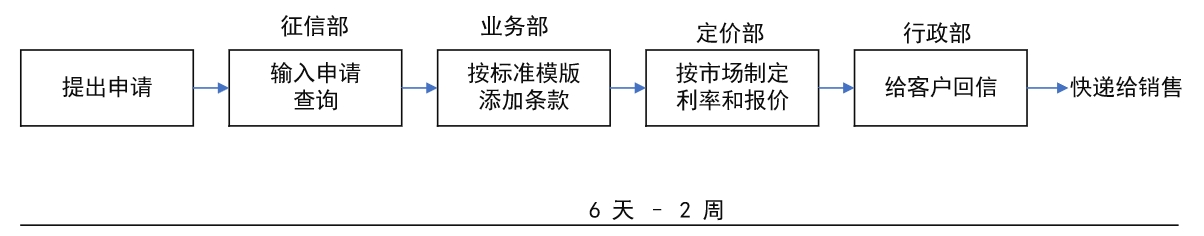
\includegraphics[width=10cm]{贷款流程图2.jpg}

前线销售觉得这时间太长，有风险（因为过程中，客户可能受竞争对手影响，改变主意），希望尽量缩短审批时间。\\
高层特意召集所有相关人员，一起模拟从头到尾的过程，发现贷款实际工作只需要90分钟。一起复盘讨论时，发现当初设计流程时以为每个环节都需要专业人士处理，但其实没有这么复杂，于是把贷款工作改为由1个人处理，并提供他一些工具与模板，发现经过培训后，整个审批流程确实可以由一个人处理。这不仅减少了人手，还把贷款单的处理效率增加了100倍。

\begin{description}
\tightlist
\item[]
(如想多了解IBM Credit故事，参考Hammer第2章)
\end{description}

\hypertarget{value-stream-map-ux4ef7ux503cux6d41ux56fe}{%
\subsection{Value Stream Map
价值流图}\label{value-stream-map-ux4ef7ux503cux6d41ux56fe}}

从以上两个例子看到重新设计业务流程能节省时间，这种思路能用于软件开发吗？\\
前面十四章提到软件开发过程有各种浪费，我们可以用价值流分析，先画出当前流程，识别哪些过程有价值，哪些是浪费？然后分析原因，优化过程。\\
价值流 (Value Stream)
是精益的过程分析方法，先画出从头到尾全流程，然后识别哪些是有价值，哪些是浪费；然后分析看如何能减少浪费。\\
下是我用于精益价值流培训的小组练习题，欢迎尝试提出你的解决方案（答案在附件）：

\framebox{%
\begin{minipage}[t]{0.97\columnwidth}\raggedright
\textbf{练习题} 某家游戏开发公司开发过程的价值流图：

%\href{文件:上市价值流图.jpg}{650px}

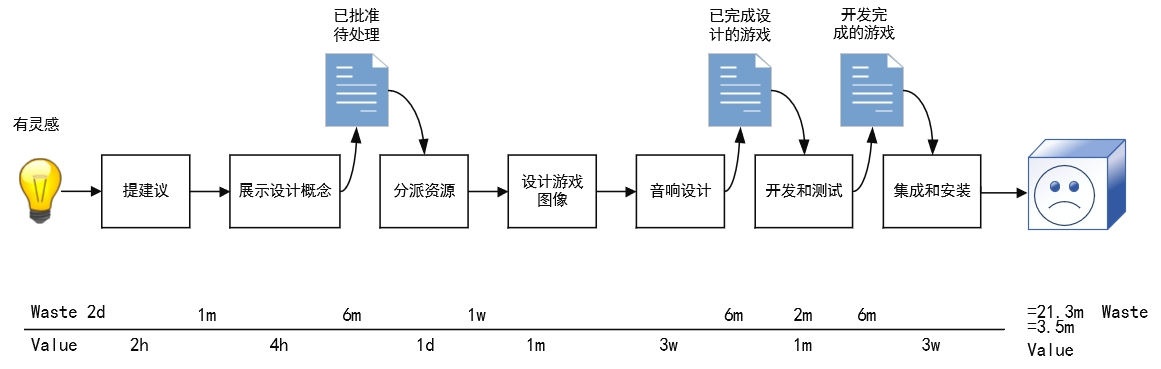
\includegraphics[width=10cm]{上市价值流图.jpg}

当有人想出新游戏的想法时，他会花几个小时准备概念演示。大约一个月后，这个想法被提交给了审查委员会，如果这个想法通过审批，因这并不是唯一的游戏好建议，它与其他游戏一样等待设计，平均6个月后能安排图像和声音设计师。\\
当某设计师有空后，主管便将新游戏分配给他们，两个月后完成设计。当游戏被设计出来后，因开发与测试资源有限，要等待（平均6个月）。当开发团队最终开始开发这款游戏时，因同时还在开发另外两款游戏，所以他们花了3个月的时间来完成开发，尽管团队只花了1个月的时间来开发这游戏。当团队完成后，游戏再等待6个月，才最终通过集成和部署安装。从最初有想法，最终经过两年，这款游戏才发行。但在这两年中，只有3个半月或14\%的时间真正用于为游戏增加价值。\\
请问有什么改进建议？
\strut
\end{minipage}}

\hypertarget{ux603bux7ed3}{%
\subsection{总结}\label{ux603bux7ed3}}

正如戴明博士说，要清除部门间的围墙，一起合作为客户服务，所以不能单靠每个子过程最优，更重要是从头到尾的效果，是否让客户满意，并减少浪费。\\
但是否设计好总体的优化系统和流程便能得到理想效果呢？下章继续。

\hypertarget{ux9644ux4ef6}{%
\section{附件}\label{ux9644ux4ef6}}

\hypertarget{ux7ec3ux4e60ux7b54ux6848}{%
\subsection{练习答案}\label{ux7ec3ux4e60ux7b54ux6848}}

这个案例出现了三类浪费：

\begin{enumerate}
\tightlist
\item
  过程中库存、半成品 (In-Process Inventory)
\item
  交接 (Handovers)
\item
  任务替换 (Task Switching, Multi-tasking)
\end{enumerate}

公司为了精简，成立了跨部门团队，每个团队只开发一款游戏，团队就可以自己把握从头到尾的整个流程，避免中间交接，例如：刚开始第一个跨功能团队，能在四个月内开发出一款新游戏，是之前开发时间的六分之一。

\hypertarget{ux53c2ux8003-references}{%
\section{参考 References}\label{ux53c2ux8003-references}}

\begin{enumerate}
\tightlist
\item
  Poppendieck, Mary, Poppendieck, Tom \emph{Leading Lean Software
  Development} (2010) Pearson Education\\
\item
  Hammer, Michael , Champy, James \emph{Reengineering the Corporation}
  (1993) Nicholas Brealey Publishing\\
\end{enumerate}


